% CacheMind -- presentation (14 frames)
% Compile: pdflatex cachemind.tex  (twice), or upload to Overleaf.

\documentclass[aspectratio=169,11pt]{beamer}

\usetheme{Madrid}
\usecolortheme{default}
\setbeamertemplate{navigation symbols}{}
\setbeamertemplate{itemize items}[circle]
\setbeamerfont{frametitle}{size=\large,series=\bfseries}

\usepackage[T1]{fontenc}
\usepackage[utf8]{inputenc}
\usepackage{booktabs}
\usepackage{listings}
\usepackage{tikz}
\usetikzlibrary{arrows.meta}
\usepackage{pgfplots}
\pgfplotsset{compat=1.16}

% ---------- colours ----------
\definecolor{cmblue}{RGB}{31,78,121}
\definecolor{cmhot}{RGB}{214,96,77}
\definecolor{cmcold}{RGB}{67,147,195}
\definecolor{cmgreen}{RGB}{77,146,33}
\definecolor{cmgrey}{RGB}{110,110,110}
\definecolor{cmbg}{RGB}{245,247,250}

% ---------- code listings ----------
\lstdefinestyle{cm}{
  language=Python,
  basicstyle=\ttfamily\scriptsize,
  keywordstyle=\color{cmblue}\bfseries,
  commentstyle=\color{cmgrey}\itshape,
  stringstyle=\color{cmhot},
  backgroundcolor=\color{cmbg},
  frame=single,
  rulecolor=\color{cmgrey!40},
  breaklines=true,
  columns=fullflexible,
  keepspaces=true,
  showstringspaces=false,
  xleftmargin=4pt,
  xrightmargin=4pt,
  aboveskip=4pt,
  belowskip=2pt
}
\lstset{style=cm}

% ---------- tikz styles ----------
\tikzset{
  box/.style={draw=cmblue, rounded corners=2pt, fill=cmbg, align=center,
              text width=1.75cm, minimum height=0.95cm, font=\scriptsize},
  hot/.style={box, draw=cmhot, fill=cmhot!12},
  cold/.style={box, draw=cmcold, fill=cmcold!14},
  ask/.style={box, draw=cmgrey, fill=white, text width=1.95cm},
  arr/.style={-{Stealth[length=2mm]}, thick, draw=cmgrey},
  lab/.style={font=\scriptsize, text=cmgrey}
}

% one-line plain-language description under a bullet
\newcommand{\say}[1]{\\ {\footnotesize\color{cmgrey}#1}}

\title[CacheMind]{CacheMind}
\subtitle{A self-learning semantic cache for RAG retrieval}
\author[Team VAAP]{Team VAAP}
\date{\today}

\begin{document}

% =====================================================================
% FRAME 1 -- Title
% =====================================================================
\begin{frame}
\titlepage
\end{frame}

% =====================================================================
% FRAME 2 -- Problem
% =====================================================================
\begin{frame}{The problem: RAG repeats expensive retrieval}
\begin{columns}[T,onlytextwidth]
\begin{column}{0.56\textwidth}
\begin{itemize}
  \setlength{\itemsep}{5pt}
  \item Every query pays again: keyword scan, embeddings, re-scoring.
        \say{The same work is repeated even for a repeated question.}
  \item Same question, different words: exact-match caches miss.
        \say{``What is a CNN?'' and ``Explain CNNs'' look different as text.}
  \item LRU / LFU track \emph{when} and \emph{how often}, never \emph{meaning}.
        \say{They cannot tell that two chunks are about the same topic.}
  \item No single eviction policy suits every workload.
        \say{What works for steady topics fails when topics change.}
\end{itemize}
\end{column}
\begin{column}{0.40\textwidth}
\begin{block}{Our idea}
\small
A small in-memory cache of document chunks, searched by meaning,
that \textbf{learns which eviction policy to trust} as queries arrive.
\end{block}
\end{column}
\end{columns}
\end{frame}

% =====================================================================
% FRAME 3 -- Architecture
% =====================================================================
\begin{frame}{Two-tier architecture}
\centering
\resizebox{0.98\textwidth}{!}{%
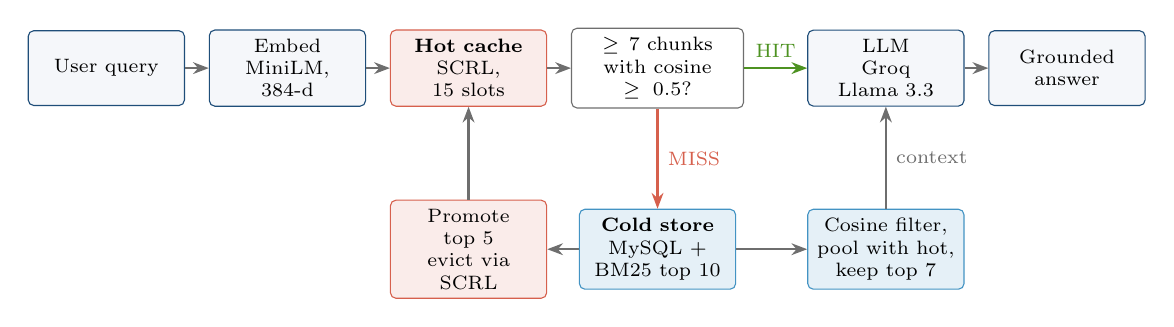
\begin{tikzpicture}
  % row 1: hit path
  \node[box]  (q)   at (0,0)     {User query};
  \node[box]  (e)   at (2.3,0)   {Embed\\MiniLM, 384-d};
  \node[hot]  (h)   at (4.6,0)   {\textbf{Hot cache}\\SCRL, 15 slots};
  \node[ask]  (d)   at (7.0,0)   {$\geq 7$ chunks with cosine $\geq 0.5$?};
  \node[box]  (l)   at (9.9,0)  {LLM\\Groq Llama 3.3};
  \node[box]  (a)   at (12.2,0)  {Grounded answer};
  % row 2: miss path
  \node[hot]  (p)   at (4.6,-2.3)  {Promote top 5\\evict via SCRL};
  \node[cold] (c)   at (7.0,-2.3)  {\textbf{Cold store}\\MySQL + BM25 top 10};
  \node[cold] (f)   at (9.9,-2.3) {Cosine filter, pool with hot, keep top 7};

  \draw[arr] (q) -- (e);
  \draw[arr] (e) -- (h);
  \draw[arr] (h) -- (d);
  \draw[arr, draw=cmgreen] (d) -- node[lab, above, text=cmgreen] {HIT} (l);
  \draw[arr] (l) -- (a);
  \draw[arr, draw=cmhot] (d) -- node[lab, right, text=cmhot] {MISS} (c);
  \draw[arr] (c) -- (f);
  \draw[arr] (f) -- node[lab, right] {context} (l);
  \draw[arr] (c) -- (p);
  \draw[arr] (p) -- (h);
\end{tikzpicture}%
}

\vspace{6pt}
\small
\textbf{Hot} = small, fast, in memory. \textbf{Cold} = every chunk, in MySQL,
searched by keywords.\\
A hit skips the BM25 scan, the cross-encoder and up to 10 chunk embeddings.
\end{frame}

% =====================================================================
% FRAME 4 -- Step by step: one question, start to end
% =====================================================================
\begin{frame}{Step by step: what happens to one question}
\small
\begin{enumerate}
  \setlength{\itemsep}{4pt}
  \item \textbf{The question comes in.} The user types it in the app.
  \item \textbf{Turn it into numbers.} A small model turns the question into
        384 numbers that capture its meaning.
  \item \textbf{Look in the hot cache first.} Compare the question with the
        15 stored chunks.
  \item \textbf{Enough matches (7 or more)?} Use them directly. This is a
        \textcolor{cmgreen}{\textbf{cache hit}}.
  \item \textbf{Not enough?} Clean and lemmatize the question, search the text
        with BM25, take the top 10. This is a
        \textcolor{cmhot}{\textbf{cache miss}}.
  \item \textbf{Keep only what fits.} Drop chunks that are not close in
        meaning; keep the best 7.
  \item \textbf{Answer.} The LLM writes the answer using only those chunks.
  \item \textbf{Update the cache.} Save the best 5 new chunks. If the cache
        is full, the policy decides what to remove.
\end{enumerate}
\end{frame}

% =====================================================================
% FRAME 5 -- Miss path: lemmatized BM25 search
% =====================================================================
\begin{frame}[fragile]{On a miss: lemmatized keyword search fills the gap}
\begin{itemize}
  \setlength{\itemsep}{3pt}
  \item Fewer than 7 cached chunks match? Fall back to BM25 text search over MySQL.
  \item spaCy drops stop words and punctuation, keeps each word \emph{and} its lemma.
  \item The top 10 BM25 chunks join the partial cache hits in one pool.
\end{itemize}
\vspace{3pt}
{\small
``What are convolutional neural networks?''
$\;\rightarrow\;$
\texttt{convolutional, neural, networks, network}\par}
\vspace{1pt}
\begin{lstlisting}
# core/cold_storage.py (condensed): lemmatize the query, then score with BM25
tokens = []
for token in self.nlp(query.lower()):
    if not token.is_stop and not token.is_punct and not token.is_space:
        tokens.append(token.text)              # the word as typed
        if token.lemma_ != token.text:
            tokens.append(token.lemma_)        # plus its base form
scores = self.bm25_index.get_scores(tokens)    # keep the top 10
\end{lstlisting}
\end{frame}

% =====================================================================
% FRAME 6 -- Admission
% =====================================================================
\begin{frame}[fragile]{Selective admission: only useful chunks get a slot}
\begin{itemize}
  \setlength{\itemsep}{3pt}
  \item BM25 matches on shared words; one common word is not relevance.
        \say{Without a filter, the cache fills up with loosely related chunks.}
  \item Admit only chunks with cosine $\geq 0.5$ to the query, top 5 per miss.
        \say{A chunk must be close in meaning, and only the best five get in.}
  \item Each promoted chunk carries its cross-encoder relevance score.
        \say{We use this score later, if removing the chunk turns out to be a mistake.}
\end{itemize}
\vspace{2pt}
\begin{lstlisting}
# app.py (condensed): rank the pooled candidates, promote the best new ones
ranked = sorted(pool.items(), key=lambda kv: kv[1]["sim"],
                reverse=True)[:HIT_THRESHOLD]
new = [(d, i) for d, i in ranked if i["embedding"] is not None]
for doc_id, info in new[:INSERT_COUNT]:
    hot_storage.insert(doc_id, info["embedding"],
                       ce_score=info["ce_score"])
\end{lstlisting}
\end{frame}

% =====================================================================
% FRAME 7 -- Cache policy: who leaves when the cache is full
% =====================================================================
\begin{frame}{Cache policy: who leaves when the cache is full?}
\begin{columns}[T,onlytextwidth]
\begin{column}{0.53\textwidth}
\small
\textbf{Three experts, three opinions}\\[3pt]
\begin{tabular}{@{}lp{5.2cm}@{}}
\toprule
\textbf{Expert} & \textbf{Wants to remove\ldots} \\
\midrule
SemLRU & the chunk least related to recent questions \\
LFU    & the chunk used the fewest times \\
RDGE   & like SemLRU, but also protects chunks similar to what cold
         search just returned \\
\bottomrule
\end{tabular}
\end{column}
\begin{column}{0.44\textwidth}
\small
\textbf{What happens, in order}
\begin{enumerate}
  \setlength{\itemsep}{2pt}
  \item The cache is full and a new chunk must enter.
  \item Each expert names one chunk to remove.
  \item We pick one expert, using the \textbf{weights}.
  \item That expert's chunk is removed.
  \item The removed chunk is noted in that expert's \textbf{ghost list}.
\end{enumerate}
\end{column}
\end{columns}
\vspace{8pt}
{\small\color{cmgrey}
If all three experts name the same chunk, nobody is blamed later: no
single expert made that choice.\par}
\end{frame}

% =====================================================================
% FRAME 8 -- How the weights are given
% =====================================================================
\begin{frame}[fragile]{How the weights are given}
\begin{columns}[T,onlytextwidth]
\begin{column}{0.57\textwidth}
\small
\begin{itemize}
  \setlength{\itemsep}{3pt}
  \item \textbf{Start equal.} Each expert gets $1/3$.
  \item \textbf{Picking.} An expert is chosen with a chance equal to its
        weight. Above 0.6, we always follow that expert.
  \item \textbf{A mistake costs weight.} If a removed chunk is needed
        again, the expert that removed it is penalised.
  \item \textbf{Never zero.} Weights always add up to 1 and stay between
        0.01 and 0.99.
\end{itemize}
\end{column}
\begin{column}{0.40\textwidth}
\small
\textbf{Worked example}\\[2pt]
\begin{tabular}{@{}lccc@{}}
\toprule
 & SemLRU & LFU & RDGE \\
\midrule
Before & 0.33 & 0.33 & 0.33 \\
After  & 0.36 & \textcolor{cmhot}{\textbf{0.27}} & 0.36 \\
\bottomrule
\end{tabular}\\[3pt]
{\footnotesize\color{cmgrey}
LFU removed a chunk. One question later we needed it again
(relevance 0.9).\par}
\end{column}
\end{columns}
\vspace{4pt}
\begin{lstlisting}
# cache/hedge.py (condensed): penalise the expert that removed a needed chunk
t      = max(0, current_time - evicted_time)     # questions since removal
reward = -(ce_score * self.discount_rate ** t)   # bigger if relevant and recent
self.W[expert_idx] *= np.exp(self.learning_rate * reward)
self.W = np.clip(self.W / self.W.sum(), 0.01, 0.99)
\end{lstlisting}
\end{frame}

% =====================================================================
% FRAME 9 -- The ghost cache
% =====================================================================
\begin{frame}{The ghost cache: remembering what we removed}
\begin{columns}[c,onlytextwidth]
\begin{column}{0.60\textwidth}
\small
\begin{itemize}
  \setlength{\itemsep}{4pt}
  \item \textbf{What it is.} One short list per expert of the chunks it
        recently removed (up to 15 each). It takes no cache slot.
  \item \textbf{Why we need it.} It is the only way to find out later
        that a removal was a mistake.
  \item \textbf{When a chunk comes back} from the cold search, we check
        the lists. Found? That expert removed something we needed, so
        its weight drops.
  \item \textbf{The chunk returns} with its old usage count plus one.
  \item \textbf{Not found?} Nobody is blamed. The oldest entries drop
        off first.
\end{itemize}
\end{column}
\begin{column}{0.37\textwidth}
\centering
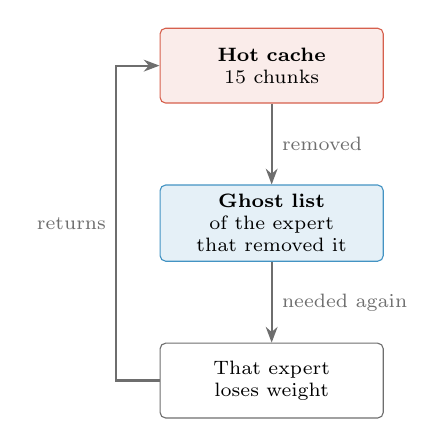
\begin{tikzpicture}
  \node[hot, text width=2.6cm]  (hc) at (0,0)    {\textbf{Hot cache}\\15 chunks};
  \node[cold, text width=2.6cm] (gl) at (0,-2.0) {\textbf{Ghost list}\\of the expert that removed it};
  \node[ask, text width=2.6cm]  (pn) at (0,-4.0) {That expert loses weight};
  \draw[arr] (hc) -- node[lab, right] {removed} (gl);
  \draw[arr] (gl) -- node[lab, right] {needed again} (pn);
  \draw[arr] (pn.west) -- ++(-0.55,0) |- node[lab, pos=0.25, left] {returns} (hc.west);
\end{tikzpicture}
\end{column}
\end{columns}
\end{frame}

% =====================================================================
% FRAME 10 -- Graded regret
% =====================================================================
\begin{frame}{Our twist: regret is graded, and fades with time}
\begin{columns}[c,onlytextwidth]
\begin{column}{0.54\textwidth}
\centering
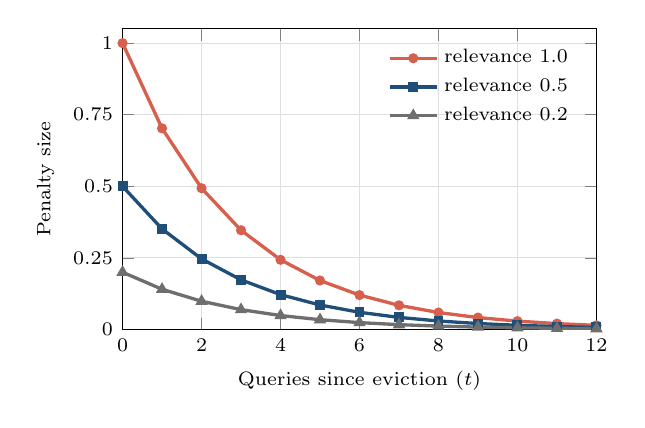
\begin{tikzpicture}
\begin{axis}[
  width=7.6cm, height=5.4cm,
  xlabel={Queries since eviction ($t$)},
  ylabel={Penalty size},
  xmin=0, xmax=12, ymin=0, ymax=1.05,
  xtick={0,2,4,6,8,10,12},
  ytick={0,0.25,0.5,0.75,1},
  grid=major, grid style={gray!25},
  label style={font=\scriptsize},
  tick label style={font=\scriptsize},
  legend style={font=\scriptsize, draw=none, fill=none,
                at={(0.97,0.97)}, anchor=north east},
  legend cell align=left
]
\addplot[cmhot, very thick, mark=*, mark size=1.2pt,
         domain=0:12, samples=13] {0.7024^x};
\addlegendentry{relevance 1.0}
\addplot[cmblue, very thick, mark=square*, mark size=1.2pt,
         domain=0:12, samples=13] {0.5*0.7024^x};
\addlegendentry{relevance 0.5}
\addplot[cmgrey, very thick, mark=triangle*, mark size=1.4pt,
         domain=0:12, samples=13] {0.2*0.7024^x};
\addlegendentry{relevance 0.2}
\end{axis}
\end{tikzpicture}
\end{column}
\begin{column}{0.43\textwidth}
\small
\[
  \text{penalty} = CE(q,d)\cdot \delta^{\,t}
\]
\begin{itemize}
  \setlength{\itemsep}{5pt}
  \item $CE$: how relevant the removed chunk really was, from 0 to 1,
        scored by a cross-encoder.
  \item $\delta \approx 0.70$: blame shrinks by about half every two
        questions.
  \item Removing an important chunk just now: big penalty.
  \item Removing noise long ago: almost none.
\end{itemize}
\end{column}
\end{columns}
\end{frame}

% =====================================================================
% FRAME 11 -- Evaluation
% =====================================================================
\begin{frame}{No single expert always wins; SCRL stays steady}
\begin{columns}[c,onlytextwidth]
\begin{column}{0.56\textwidth}
\centering
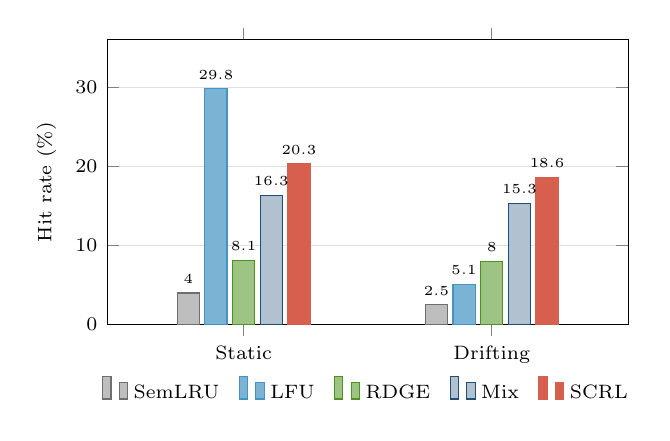
\begin{tikzpicture}
\begin{axis}[
  ybar, bar width=8pt,
  width=8.2cm, height=5.2cm,
  ymin=0, ymax=36,
  ylabel={Hit rate (\%)},
  symbolic x coords={Static,Drifting},
  xtick=data,
  enlarge x limits=0.55,
  ymajorgrids, grid style={gray!25},
  label style={font=\scriptsize},
  tick label style={font=\scriptsize},
  nodes near coords,
  every node near coord/.append style={font=\tiny},
  legend style={font=\scriptsize, draw=none, fill=none,
                at={(0.5,-0.16)}, anchor=north, legend columns=5,
                /tikz/every even column/.append style={column sep=5pt}}
]
\addplot[fill=cmgrey!45, draw=cmgrey] coordinates {(Static,4.0) (Drifting,2.5)};
\addplot[fill=cmcold!70, draw=cmcold] coordinates {(Static,29.8) (Drifting,5.1)};
\addplot[fill=cmgreen!55, draw=cmgreen] coordinates {(Static,8.1) (Drifting,8.0)};
\addplot[fill=cmblue!35, draw=cmblue] coordinates {(Static,16.3) (Drifting,15.3)};
\addplot[fill=cmhot, draw=cmhot] coordinates {(Static,20.3) (Drifting,18.6)};
\legend{SemLRU,LFU,RDGE,Mix,SCRL}
\end{axis}
\end{tikzpicture}
\end{column}
\begin{column}{0.41\textwidth}
\small
\begin{itemize}
  \setlength{\itemsep}{5pt}
  \item LFU leads on a static workload, then drops to 5\% under drift.
  \item SCRL holds about 20\% on both: $2.3\times$ the best single
        expert under drift.
  \item Learning adds 3--4 points over an unweighted mix of the same
        experts.
\end{itemize}
\vspace{3pt}
{\scriptsize\color{cmgrey}
Synthetic trace, eviction logic only: 40 topics, Zipf popularity,
2000 queries, mean of 10 seeds. Same cache classes and thresholds
as the app; cosine stands in for the cross-encoder score.
Mix = the three experts with equal, frozen weights.\par}
\end{column}
\end{columns}
\end{frame}

% =====================================================================
% FRAME 12 -- Journey
% =====================================================================
\begin{frame}{How we got here: seven steps in six weeks}
\centering
\resizebox{0.98\textwidth}{!}{%
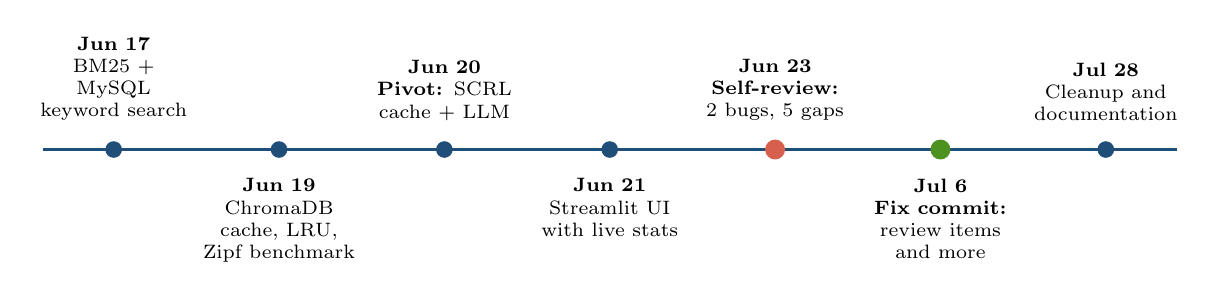
\begin{tikzpicture}
  \draw[very thick, draw=cmblue] (0,0) -- (14.4,0);
  \tikzset{ev/.style={align=center, text width=1.95cm, font=\scriptsize}}
  \fill[cmblue] (0.9,0) circle (3pt);
  \node[ev, above=7pt] at (0.9,0) {\textbf{Jun 17}\\BM25 + MySQL keyword search};
  \fill[cmblue] (3.0,0) circle (3pt);
  \node[ev, below=7pt] at (3.0,0) {\textbf{Jun 19}\\ChromaDB cache, LRU, Zipf benchmark};
  \fill[cmblue] (5.1,0) circle (3pt);
  \node[ev, above=7pt] at (5.1,0) {\textbf{Jun 20}\\ \textbf{Pivot:} SCRL cache + LLM};
  \fill[cmblue] (7.2,0) circle (3pt);
  \node[ev, below=7pt] at (7.2,0) {\textbf{Jun 21}\\Streamlit UI with live stats};
  \fill[cmhot] (9.3,0) circle (3.6pt);
  \node[ev, above=7pt] at (9.3,0) {\textbf{Jun 23}\\ \textbf{Self-review:} 2 bugs, 5 gaps};
  \fill[cmgreen] (11.4,0) circle (3.6pt);
  \node[ev, below=7pt] at (11.4,0) {\textbf{Jul 6}\\ \textbf{Fix commit:} review items and more};
  \fill[cmblue] (13.5,0) circle (3pt);
  \node[ev, above=7pt] at (13.5,0) {\textbf{Jul 28}\\Cleanup and documentation};
\end{tikzpicture}%
}

\vspace{8pt}
\small
\begin{columns}[T,onlytextwidth]
\begin{column}{0.47\textwidth}
\textbf{Why we pivoted (Jun 20)}\\
A fixed policy is a guess about the workload. We let the cache learn it.
\end{column}
\begin{column}{0.49\textwidth}
\textbf{Why we paused (Jun 23)}\\
The first app ran end to end, but the cache rarely hit and filled
with noise. We audited it before adding anything else.
\end{column}
\end{columns}
\end{frame}

% =====================================================================
% FRAME 13 -- From the Jun 23 review to the final system
% =====================================================================
\begin{frame}{Jun 23 review: what we found, what we shipped}
\footnotesize
\renewcommand{\arraystretch}{1.18}
\begin{tabular}{@{}p{4.5cm}p{3.7cm}p{4.9cm}@{}}
\toprule
\textbf{Found in our own review} & \textbf{We proposed} & \textbf{Final system} \\
\midrule
A hit needed 10 matching chunks & Lower the rule to 1 &
  \textcolor{cmgreen}{Tunable rule: 7 of 15 slots} \\
Unanimous evictions still blamed one expert & Remove the extra check &
  \textcolor{cmgreen}{Done as proposed} \\
Every cold result was cached & Freq-K or similarity gate &
  \textcolor{cmgreen}{Cosine $\geq 0.5$ gate, top 5 per miss} \\
Penalty score was always 1.0 & Cosine as a proxy &
  \textcolor{cmgreen}{Went further: real cross-encoder} \\
SemLRU ignores recency & Blend in recency &
  \textcolor{cmgrey}{Next step} \\
Hedge turns greedy above 0.6 & Temperature sampling &
  \textcolor{cmgrey}{Next step} \\
Fallback ignores the weights & Weight-guided pick &
  \textcolor{cmgrey}{Dropped: that path never runs} \\
\bottomrule
\end{tabular}

\vspace{6pt}
\small
\textbf{Then the UI exposed more, fixed in the same commit:} two cache
lookups per miss, counters that disagreed, invisible evictions.
\end{frame}

% =====================================================================
% FRAME 14 -- What stands out + next steps
% =====================================================================
\begin{frame}{What makes CacheMind stand out}
\begin{columns}[T,onlytextwidth]
\begin{column}{0.60\textwidth}
\small
\begin{itemize}
  \setlength{\itemsep}{3pt}
  \item \textbf{Caches evidence, not answers}
        \say{Every reply is still written from the real source text.}
  \item \textbf{The cache learns its own rule}
        \say{LeCaR-style online learning, applied to meaning-based data.}
  \item \textbf{Mistakes are graded}
        \say{A cross-encoder decides how costly each wrong removal was.}
  \item \textbf{Cold search guides eviction}
        \say{RDGE protects chunks similar to what BM25 just returned.}
  \item \textbf{Cheap cold tier}
        \say{Lemmatized BM25 on MySQL: no vector database needed.}
  \item \textbf{Glass-box demo}
        \say{Every hit, miss and removal is shown with its reason.}
\end{itemize}
\end{column}
\begin{column}{0.36\textwidth}
\begin{block}{Next steps}
\small
\begin{itemize}
  \item Recency-aware SemLRU
  \item Softer Hedge sampling
  \item Benchmark on real query logs
\end{itemize}
\end{block}
\vspace{6pt}
\centering
{\large\bfseries\color{cmblue} Thank you}\\[2pt]
{\small Questions?}
\end{column}
\end{columns}
\end{frame}

\end{document}
